\section{Introduction}

Recent years have witnessed widespread use of sophisticated frameworks such as Dryad\cite{dryad}, Spark\cite{spark} and Apache Tez\cite{tez}.
Tremendous effeorts have been paid to improve the speed and of large-scale dataparallel systems computing process, from the the low level storage system to scheduling algorithms.

% take over shuffle
%shuffle characteristic
DAG computing framworks deriving from MapReduce\cite{mapreduce} contains a hard barrier between computing stages. The terminology of this barrier is \textit{shuffle}. Shuffle contains two parts on the connecting stages -- \textit{shuffle write} and \textit{shuffle read}. On the side of ancestor stages, \textit{shuffle write} is resoponsible for writing intermediate results to disk. On the side of descendant stage, \textit{shuffle read} fetches intermediate results from remote disks through network. Although highly optimized in other factors, the shuffle of framework is still primitive.  The coarse design of shuffle introduce a significiant performance overhead.
% design inconsistent
For instance, a MapReduce trace analysis from Facebook shows that shuffle accounts for 33\% JCT on average, up to 70\% in shuffle-heavy jobs\cite{managing}.
% shuffle operations
% three resource coordinate 不好
% 计算和I/O couple, why
% why disk, reason!!!, 不重视
% common problems

The main defect of current shuffle design is coarse granularity of resource allocation during the task scheduling. 
Nearly all task scheduling algorithms in DAG frameworks use time slotted model. Specifically, when a task is launched, the framework offers it a bundle of resources (i.e. CPU and memory), which are dedicated to this task during the time in its "slot". 
But for a task, the resources demand changes during different phases. The computing phase is CPU and memory intensive. The shuffle, instead, is I/O intensive. 
As shown in the upper part of Figure \ref{fig:workflow}, this "slot" can be released until the map tasks finish \textit{shuffle write} on disk. And the "slot" is occupied when the reduce tasks begin to read shuffle data from remote nodes through network, which is presented as \textit{shuffle read}. This inconsistency between demands and allocation results in a severe resource underutilization, which slow down the framework.

Another drawback of current shuffle is the synchronized shuffle read. When all the reduce tasks are scheduled, the shuffle fetch of each task starts almost simultaneously, which may cause congestion of network and delay the shuffle read. The straight forward way to avoid network burst is to start reduce tasks earlier. Apache Hadoop\cite{hadoop} provides a mechanism that schedules reduce tasks when a certain portion of map tasks completed. So that the shuffle delay can be mitigated. Other publications also purpose solutions to pre-schedule reduce tasks\cite{ihadoop, ishuffle, dynmr}. However this early scheduling of reduce tasks occupies new task slots, which degrades system performance. To this end, we proposed a question for this cross-frameworks issue, \textit{can we efficiently optimize shuffle without manually change every DAG framework?} 

\begin{figure}
	\centering
	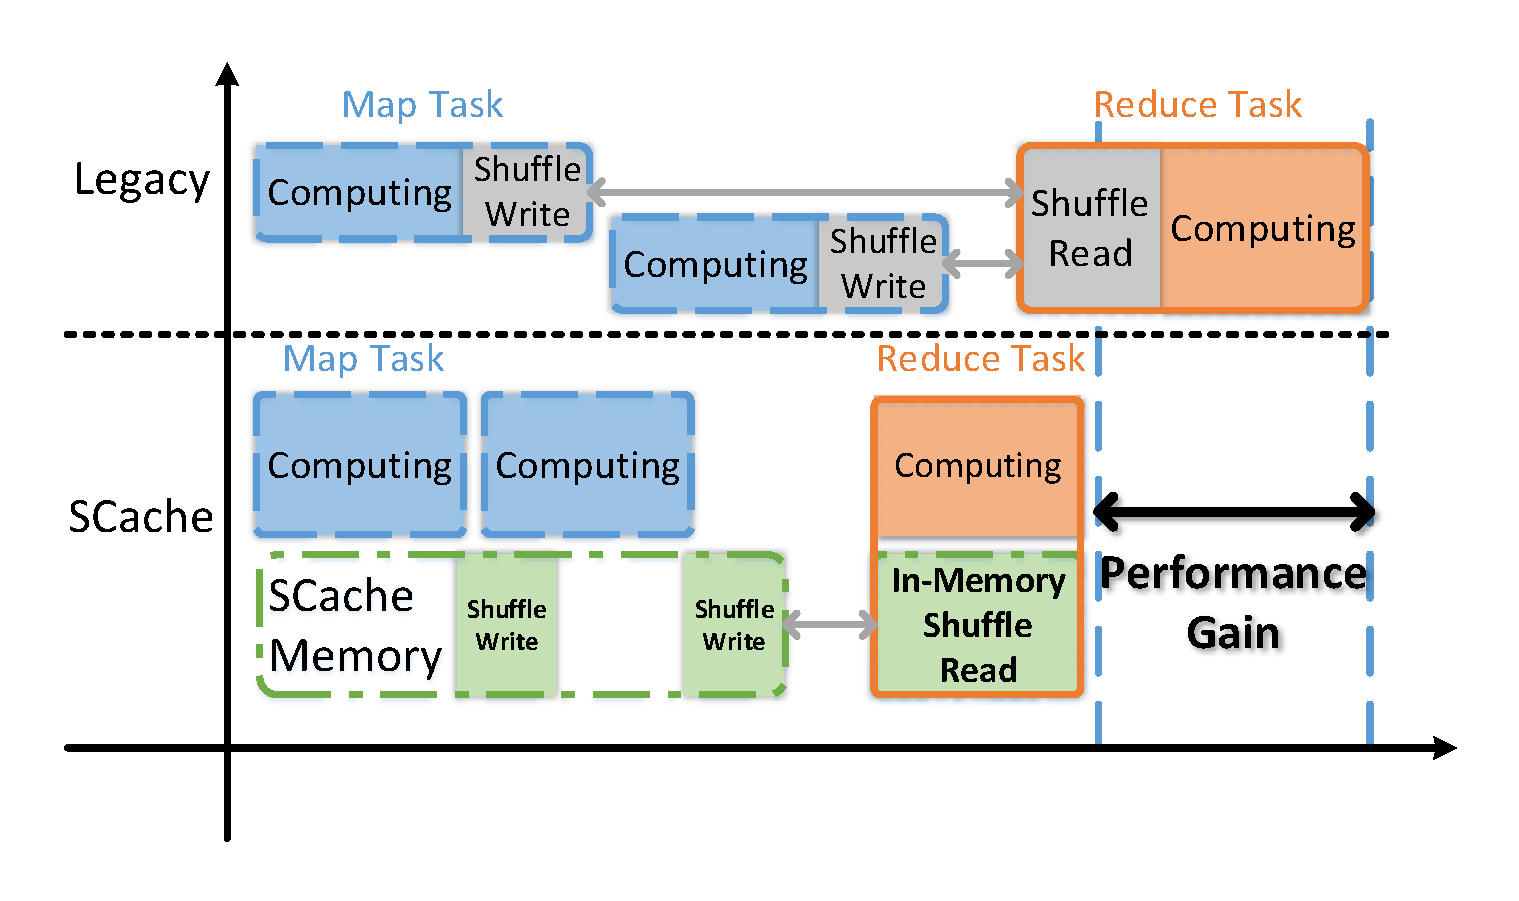
\includegraphics[width=\linewidth]{fig/workflow}
	\caption{Workflow Comparison between Legacy DAG Computing Frameworks and Frameworks with SCache}
	\label{fig:workflow}
\end{figure}


% 针对性的提出这三个点
% three resource coordinate 不好
% 计算和I/O couple, why
% why disk, reason, 不重视
% common problems
% 总起:普适性工具
% pre-fetch but not pre-execute
% byproduct: more balance
% memory instead of disk

% challenge point by point, inside the problem

In this paper, we introduce S(huffle)Cache, an plugin system to remove shuffle latency for DAG frameworks. SCache takes over the management of shuffle and I/O resources to acheive a fine granularity scheduling of tasks. In addition, SCache pre-schedules the reduce tasks without launching them and perform shuffle data pre-fetch to break the synchronization of shuffle fetch. In order to provide a general optimization for different DAG frameworks, SCache decouple the shuffle process from computing and  provide a cross-frameworks API for shuffle write and read. 

The workflow of DAG framework with SCache is presented in Figure \ref{fig:workflow}. In Figure \ref{fig:workflow}, SCache hijacks the intermediate data of a map task from memory space of the slot. The disk operation is skipped and the slot is released after the memory copy. The in-memory intermediate data is immediately shuffled through network to the remote node after heuristic pre-scheduling. By releasing the slot earlier and taking over the I/O operation to start the network transfer ahead of reduce tasks, SCache can help the DAG framework achieve a significant performance gain. A by-product optimization of heuristic pre-scheduling is that SCache can provide a more balanced load for each node. It can further benifit the reduce stage by avoiding data skew.

The main challenge to achieve this optimization is \textit{pre-scheduling reduce tasks}. This challenge is not critical for the simple DAG computing such as Hadoop MapReduce\cite{mapreduce}. Unfortunately the complexity of DAG can amplify the defects of na\"{i}ve pre-scheduling schemes. In particular, randomly assign reduce tasks to nodes can result in a collision of two heavy tasks on one node. This collision can aggravate data skew and hurts the performance of the DAG frameworks. To address this challenge, we propose a heuristic scheme to predict the shuffle output distribution and schedule reduce tasks.

The second challenge is the \textit{limitation of memory space}. To prevent shuffle data touching the disk, SCache leverages extra memory to store the shuffle data. However, the memory is a precious resource for DAG computing, especially for in-memory framework such as Spark\cite{spark}. In order to optimize shuffle without hurting the performance of DAG frameworks, SCache only reserves small fraction of memory to store shuffle data. To maximum the performance gain of optimization and memory utilization, we propose two constraints: all-or-nothing and context-aware. The memory management scheme follows these two contraints to switch shuffle data blocks on and off reserved memory.

We have implemented SCache and customized Apache Spark\cite{apachespark}. The performance of SCache is evaluated with both simulations and testbed experiments on a 50-node Amazon EC2 cluster. We conduct basic test like GroupByTest.We also evaluate benchmark like Terasort\cite{spark-tera} and standard workloads like TPC-DS\cite{tpcds} for multi-tenant modeling. In a nutshell, SCache can eliminate explict shuffle process by at most $89\%$ in varied application scenarios.




